% Section content template for individual Educative lessons
% This file contains the actual content for a specific section
% Generated from Educative API section content

% Section: Detailed Design of the Typeahead Suggestion System
% Section ID: 5464491722801152
% Section Slug: detailed-design-of-the-typeahead-suggestion-system
% Generated: 2025-12-08T15:11:37.236733

\subsection{Detailed design}\label{geGlxjTO7jA8FbJEaAXb3}
\\
Let's go over the flow and interaction of the components shown in the illustration below. Our design is divided into two main parts:

\begin{itemize}
\item
\protect\phantomsection\label{DeqBVf6bz5dv_gy0VFRT1}
A suggestion service
\item
\protect\phantomsection\label{tvkehkb14DICHwSARx4D8}
An assembler
\end{itemize}

\begin{figure}[htbp]
 \centering
 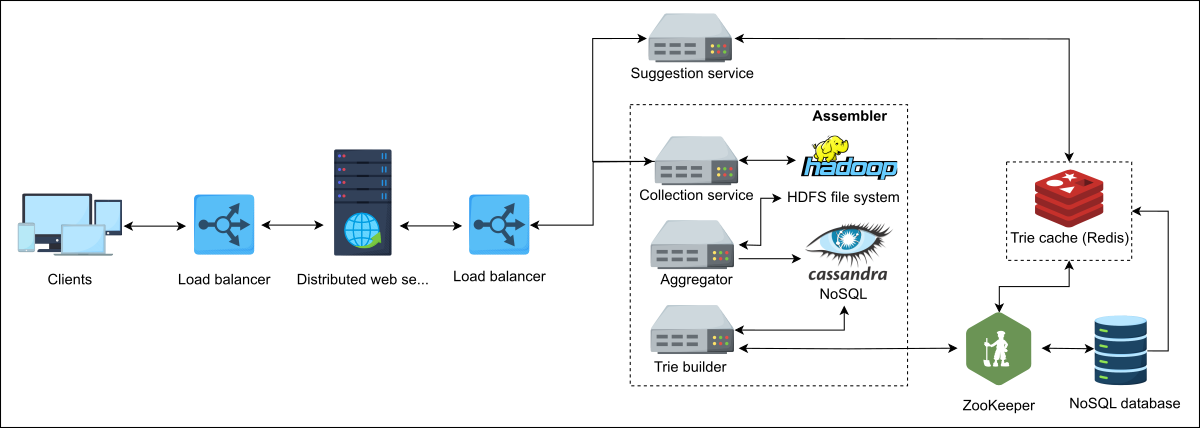
\includegraphics[width=0.5\textwidth]{Images/chapter_37/section_5464491722801152/5068440778178560.png}
 \caption{The detailed design of the typeahead suggestion system}
\end{figure}

\subsubsection{Suggestion service}\label{nstLvAUYCzn344R3SVzs9}
\\
At the same time that a user types a query in the search box, the \texttt{getSuggestions(prefix)} API calls hit the suggestions services. The top ten popular queries are returned from the distributed cache, Redis.

\subsubsection{Assembler}\label{0jd1cFVCrLkeocZq3BQ1B}
\\
In the previous lesson, we discussed how tries are built, partitioned, and stored in the database. However, the creation and updation of a trie shouldn't come in the critical path of a user's query. We shouldn't update the trie in real time for the following reasons:

\begin{itemize}
\item
\protect\phantomsection\label{PTv6aTCsTCyFFj7WOWS5Z}
There could be millions of users entering queries every second. During such phases with large amounts of incoming traffic, updating the trie in real time on every query can slow down our \textbf{suggestion service}.
\item
\protect\phantomsection\label{vE4yana_NYVHAB9bgkiYc}
We have to provide top suggestions that might not frequently change after the creation or updation of the trie. So , it's less important to update the trie frequently.
\end{itemize}
\\
In light of the reasons given above, we have a separate service called an assembler that's responsible for creating and updating tries after a certain configurable amount of time. The assembler consists of the following different services:

\begin{itemize}
\item
\protect\phantomsection\label{RZmVbS3JZ3oApyFFYE7Ie}
\textbf{Collection service:} Whenever a user types, this service collects the log that consists of phrases, time, and other metadata and dumps it in a database that's processed later. Since the size of this data is huge, the \textbf{Hadoop Distributed File System (HDFS)} is considered a suitable storage system for storing this raw data. An example of the raw data from the collection service is shown in the following table. We record the time so that the system knows when to update the frequency of a certain phrase.
\end{itemize}

\textbf{Raw Data Collected by the Collection Service}

\begin{table}[htbp]
\centering
\small
\adjustbox{max width=\textwidth}{
\begin{tabular}{|p{0.421\textwidth}|p{0.529\textwidth}|}
\hline
\textbf{Phrases} & \textbf{Date and Time (DD-MM-YYYY HH: MM: SS)} \\
\hline
\hline
UNIVERSAL & 23-03-2022 10:16:18 \\
\hline
UNIVERSITY & 23-03-2022 10:20:11 \\
\hline
UNIQUE & 23-03-2022 10:21:10 \\
\hline
UNIQUE & 23-03-2022 10:22:24 \\
\hline
UNIVERSITY & 23-03-2022 10:25:09 \\
\hline
\end{tabular}
}
\caption{Raw Data Collected by the Collection Service}
\end{table}

\begin{itemize}
\item
\protect\phantomsection\label{scxfGm_jhw7JxTF9K478W}
\textbf{Aggregator:} The raw data collected by the \textbf{collection service} is usually not in a consolidated shape. We need to consolidate the raw data to process it further and to create or update the tries. An aggregator retrieves the data from the HDFS and distributes it to different workers. Generally, the MapReducer is responsible for aggregating the frequency of the prefixes over a given interval of time, and the frequency is updated periodically in the associated Cassandra database. \textbf{Cassandra} is suitable for this purpose because it can store large amounts of data in a tabular format. The following table shows the processed and consolidated data within a particular period. This table is updated regularly by the aggregator and is stored in a hash table in a database like Cassandra. For simplicity, we assume that our data is case insensitive.
\end{itemize}

\textbf{Useful Information Extracted from the Raw Data}

\begin{table}[htbp]
\centering
\small
\adjustbox{max width=\textwidth}{
\begin{tabular}{|p{0.317\textwidth}|p{0.317\textwidth}|p{0.317\textwidth}|}
\hline
\textbf{Phrases} & \textbf{Frequency} & \textbf{Time Interval} \\
\hline
\hline
UNIVERSAL & 1400 & 1st 15 minutes \\
\hline
UNIVERSITY & 1340 & 1st 15 minutes \\
\hline
UNIQUE & 1200 & 1st 15 minutes \\
\hline
\end{tabular}
}
\caption{Useful Information Extracted from the Raw Data}
\end{table}

\begin{itemize}
\item
\protect\phantomsection\label{GkJazt1HyjH12ShATilhj}
\textbf{Trie builder:} This service is responsible for creating or updating tries. It stores these new and updated tries on their respective shards in the trie database via ZooKeeper. Tries are stored in persistent storage in a file so that we can rebuild our trie easily if necessary. NoSQL document databases such as MongoDB are suitable for storing these tries. This storage of a trie is needed when a machine restarts. The trie is updated from the aggregated data in the Cassandra database. The existing snapshot of a trie is updated with all the new terms and their corresponding frequencies. Otherwise, a new trie is created using the data in the Cassandra database. Once a trie is created or updated, the system makes it available for the suggestion service.
\end{itemize}
\\
Let\textquotesingle s assess your understanding by responding to the question below:
\\
How would you handle misspelled or incomplete words in the Typeahead Suggestion System?

\begin{quote}
\textbf{Quiz:}
\textbf{Question 1:} Should we collect data and build a trie per user, or should it be shared among all users?
\textbf{Answer:} Since we aim to design a system on a scale that's similar to Google

Search, billions of users will be using our service. Since the number of users would be huge, maintaining a tree for each user would become complex and time-consuming. There's also a possibility of duplicated trees if several users have typed some common searches, resulting in resource wastage. Therefore, our design assumes a common trie that's shared among users, where the ranking would be based on single phrases in the trie and the frequency of the terms.
\end{quote}

% End of section content